\section{Kinect Software}\label{Software}

%(Essenz auf dem, was Kinect für mich erledigt theorie, mathematische Berechnung tiefe und skeletonstream usw)


%
%		Joints
%			20 pro Skelett
%		Bone Sequence
%
%		Kinect Raum (Koord.)
%			+ Bild
%		
%		Skeleton Smoothing, Jitter
%
%	Fazit: Habe Skelett. Extrahiere Winkel, Gebe Nao




Die im vorherigen Kapitel aufgezeigte Hardware liefert die entsprechenden Sensorinformationen, die nun
softwaretechnisch zu einer abstrakteren Ebene zusammengefasst werden müssen. Die Funktion dieser
Verarbeitungen - speziell für das Microsoft Kinect SDK - soll in diesem Kapitel erläutert werden.

\begin{description}
	\item[Die Hardware liefert folgende Werte:]~\par
	\begin{itemize}
		\item RGB Bildsignal der Kamera
		\item Tiefenwerte
		\item Audiosignale inkl. Richtungswert des Microphonarrays
	\end{itemize}
\end{description}

\noindent
Wie bereits erwähnt sind die Audiodaten für dieses Projekt jedoch irrelevant. Wichtig sind primär die Bilddaten inklusive der Tiefenwerte.
Das Kinect SDK bietet bereits standardmäßig Zugriff auf diese Zahlen. Dabei können im Programm bestimmte Proxyobjekte registriert und abgefragt werden. Wie diese im Programm letztendlich verwendet werden,
wird im folgenden Kapitel \myref{SDK} näher erläutert. Dieses Kapitel beschäftigt sich
damit, wie diese Funktionen im Inneren funktionieren.

%	Depth Stream
%		43 Grad vertikal, 57 horizonzal
%		RAW Data Array (KINECT FOR WINDOWS SDK PROG GUIDE)
%			16 Bit Graustufenarray
%				Wert beschreibt Abstand zu Kinect in mm
%				Untere 3 Bits = Player Index
%				Oberen 13 Bits = Distance in mm
%
%		Depth-Range (u.a. auch Near Mode)			
%			Bild mit Werten kinect_range.png (http://msdn.microsoft.com/en-us/library/hh973078.aspx)		
%
%		Grundlage für Skeleton Stream
%			Überleitung
%
\subsection{Der Tiefenstream}
Der Tiefenstream (Depth-Stream) liefert zu jedem Pixel im Sichtfeld (43 Grad vertikal, 57 Grad horizontal) einen Tiefenwert. Dieser Wert enthält die Entfernung in Millimetern zu dem jeweiligen Objekt.
Damit ist das am nächsten befindliche Objekt gemeint, da verdeckte Objekte nicht vom Sensor erkannt werden.
Aus diesem Stream kann man beispielsweise ein Tiefenbild mit verschiedenen Farbwerten generieren, die repräsentativ für die Entfernung zur Kinect stehen (siehe Abb. \ref{f:kinect_depth_stream}). Die Depth-Stream Daten werden in einem 16 Bit Array transportiert. Dabei sind die drei untersten Bits jedoch für die Erkennung von mehreren Spielern reserviert
(Siehe Kapitel \myref{skeleton}). Die oberen 13 Bit enthalten die eigentlichen Tiefendaten. Ein solcher Tiefenstream kann wie folgt aussehen:

\begin{figure}[H]						
	\centering							
	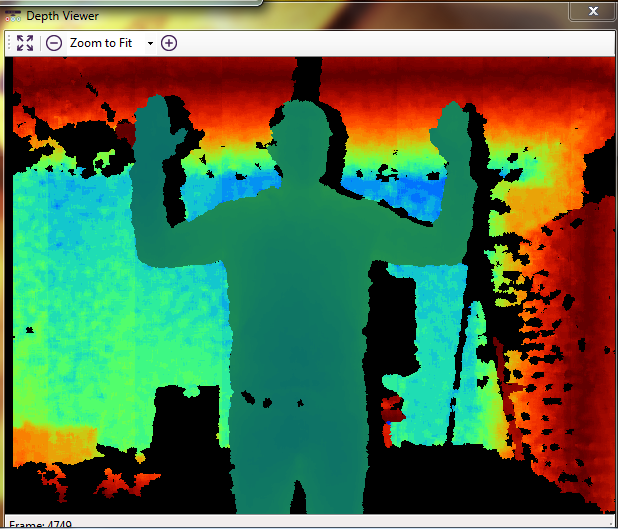
\includegraphics[scale=0.5]{Bilder/kinect_tiefenstream.png}			
	\caption{Kinect Tiefenstream}						
	\label{f:kinect_depth_stream}						
\end{figure}

Zur Erfassung eines Objektes, muss sich dieses im Sichtfeld der Kinect befinden. 
\begin{figure}[H]						
	\centering							
	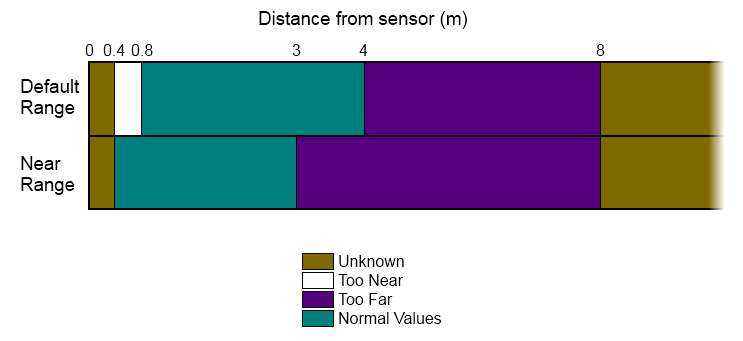
\includegraphics[scale=0.7]{Bilder/kinect_range.png}			
	\caption{Depth Space Range \cite{ws:microsoft_coordinateSpaces}}						
	\label{f:kinect_range}						
\end{figure}

Somit liegt der Arbeitsraum der Kinect im normalen Modus zwischen 0.8m und 4m. Der Near-Modus hat einen Arbeitsbereich von 0.4m - 3m. Im Laufe unseren Projektes beschränken wir uns auf den normalen Modus.

Anhand dieses Tiefenstreams ist es nun möglich Spieler (Menschen) zu extrahieren und deren Bewegungen
in Echtzeit zu erfassen. Kinect bietet durch dessen SDK bereits eine Möglichkeit, diese Daten zu
aufzuzeichnen und auszuwerten. Da das fertige Objekt durch ein Skelett dargestellt wird, ist dies auch als Skeleton-Objekt oder einfach nur als Skeleton bezeichnet. Für dieses Projekt ist dieses Skeleton-Objekt von großer Bedeutung. Anhand von Vergleichsmustern erzeugt die Software -nicht Kinect!- einen sog. Skeletonstream, der versucht die Position eines menschlichen Skeletts im Kinect Koordinatenraum abzubilden.\cite{SWB-376536934}
Wie genau dies funktioniert wird im folgenden Kapitel erläutert.



%	Skeleton Stream
%		+ Bild
% 		Benutzt Tiefenstream
%		2 Player mit allen Joints
%		Anforderung an Erkennung
%			Verschiedene Menschen, größen
%			Kleider und Farben
%			Echtzeit!
%		Erkennungsalgorithmus
%			Tiefendaten in die Rendering Pipeline
%			Labeling der Körperteile durch Segmentierung mit Farben (PDF HOW DOES KINECT WORK)
%				Spieler segmentieren (Körper >ja</nein)
%				Decition Tree Struktur = Decition Forest (Maschinell trainiert)
%					Motion Capture (MCAP) Daten Beispiele (echt)
%					Parameter
%						Größe, Breite
%						Kleidung
%						Perspektive
%					Syntetisierte Daten (Zufaellige Parameter)
%				Körpersegmente extrahieren
%			Platzierung der Joints		
%			Sensor berechnet 3D View für Gelenkkoordinaten
%				Vorne
%				Seite	
%				Oben
%
%		Mehrere Spieler (Playerindex)
%			Bis zu 6 Spieler erkennbar (Index aus Tiefenarray extrahierbar)
%			Funktioniert nur mit Skeleton Stream
%			Irrelevant für Projekt
%
\subsection{Der Skeletonstream}\label{skeleton}
Damit ein Benutzer und dessen Bewegungen mittels Kinect erkannt und im Programm verarbeitet werden können, wird der Tiefenstream entsprechend ausgewertet. Als Ergebnis erhält man ein menschliches Skelett, das aus
20 Gelenken (Joints) besteht. Diese Joints sind im Skeletonobjekt hierarchisch von der Hüfte aus miteinander verbunden und bilden somit das Skelett eines Spielers. Die folgende Grafik illustriert alle erkannten Gelenke und deren Positionen. Für dieses Projekt sind insbesondere die Joints \textit{Shoulder}, \textit{Elbow}, \textit{Wrist} und \textit{Hip} von hoher Bedeutung, da mit ihnen die Winkel der Gliedmaßen errechnet werden können (Siehe Kapitel \myref{algo_angle}).

\begin{figure}[H]						
	\centering							
	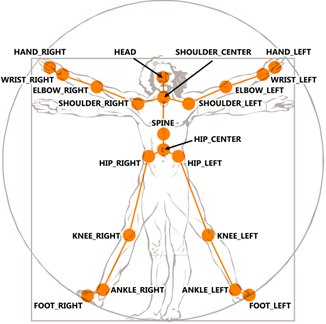
\includegraphics[scale=1.0]{Bilder/kinect_joints.png}			
	\caption{Kinect Joints \cite{ws:microsoft_jointType}}						
	\label{f:kinect_joints}						
\end{figure}

Ein Kinectsystem kann bis zu 6 Spieler gleichzeitig erkennen, wobei nur von zwei Spielern die exakte Position aller Gelenkwinkel erkannt werden kann. Von den anderen vier Spielern wird nur die Position im Raum ermittelt, nicht jedoch die exakten Koordinaten aller 20 Joints. Wie schon im vorigen Kapitel erwähnt, wird einem Spieler nach dessen Erkennung ein Index zugeordnet. Dieser befindet sich im Tiefenarray, falls die Skeletonfunktion aktiviert wurde. Innerhalb dieses Projektes ist dieser jedoch irrelevant, da angenommen wird, dass immer nur ein Spieler
den Roboter steuern wird.\\ \\
\noindent
\textbf{Skelettextraktion}\\
Hinter der Extraktion des Skeletts steckt ein Algorithmus, der bereits im \textit{Microsoft Kinect SDK} vorhanden ist. 
Die Anforderungen an diesen Algorithmus sind hoch, denn er soll Menschen mit verschiedenen Größen,
Breiten und Kleidern in Echtzeit erkennen.
Damit dies überhaupt möglich ist, wird maschinelles Lernen verwendet. Zunächst werden die aufgenommenen Tiefendaten in eine sog. \textit{Rendering Pipeline}\cite{pdf:realtime_human_pose} gegeben. Diese vergleicht die aufgenommenen Daten mit bereits
vorhandenen Beispielen, die mit verschiedenen Menschen aufgenommen wurden. Anhand eines Decision Trees, der durch maschinelles Lernen erzeugt wurde, wird ein Pixel mit einer gewissen Wahrscheinlichkeit zu einem Körpersegment zugeordnet. Der Algorithmus arbeitet zur Erhöhung der Genauigkeit mit mehreren Bäumen gleichzeitig. Somit können die Körpersegmente zugeordnet werden, was in der folgenden Grafik farbig dargestellt wird.

\begin{figure}[H]						
	\centering							
	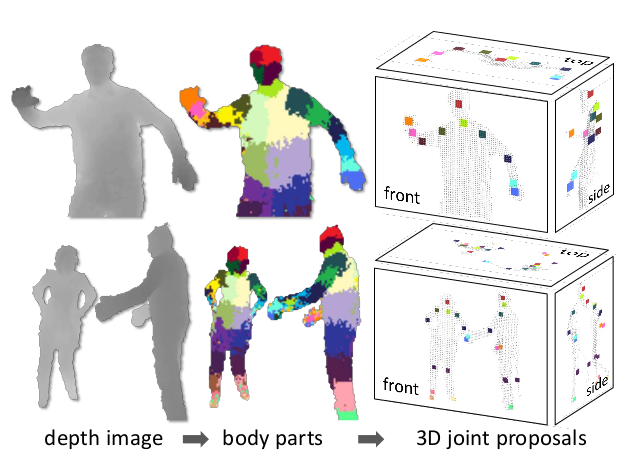
\includegraphics[scale=0.5]{Bilder/kinect_body_parts.png}			
	\caption{Skelett-Erkennung \cite{pdf:realtime_human_pose}}						
	\label{f:kinect_skeleton}						
\end{figure}

\noindent
Nach der Segmentierung werden die Gelenke innerhalb den entsprechenden Bereichen platziert. Dies wird anhand einer Häufigkeitsanalyse von Beispieldaten errechnet.
Im Anschluss daran wird ein 3D-Modell des Skeletts erstellt, das aus der \textit{Frontansicht}, der \textit{Seitenansicht} und der \textit{Draufsicht} besteht (Siehe Abb. \ref{f:kinect_skeleton} rechts: 3D joint proposals).
Dieser komplexe Prozess ermöglicht es eine Skelett-Erkennung in Echtzeit durchzuführen. Als Entwickler einer Kinect Applikation muss man sich nicht mehr um diese Erkennung kümmern, denn diese  ist bereits implementiert.
Die Koordinaten der Skeleton-Joints befinden sich im Skeletonobjekt und können mit der erkannten Genauigkeit ausgelesen und verwendet werden.
\\ \\
\textbf{Skelett-Koordinatenraum}\\
Der Koordinatenraum der Kinect ist wie folgt definiert:

\begin{figure}[H]						
	\centering							
	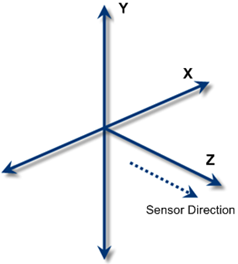
\includegraphics[scale=0.8]{Bilder/kinect_skeleton_space.png}			
	\caption{Skelett-Koordinatenraum\cite{ws:microsoft_coordinateSpaces}}						
	\label{f:kinect_skeleton_space}						
\end{figure}

\noindent
Das Kinect-Koordinatensystem ist ein rechtshändiges Koordinatensystem. Die positive Z-Richtung entspricht der Blickrichtung der Kinect. Die positive X-Richtung zeigt nach links und entsprechend die positive Y-Richtung nach oben. \cite{ws:microsoft_coordinateSpaces}

% (Bild mehrere User im Kinectraum)
%\todo{Screenshot von Deep Stream (Kinect Studio)}
%\todo{Unterschied Microsoft SDK und Freie Implementierung OpenNI}
%\todo{Bild von Kinect-Koordinatensystem -> Bezug auf Nao}
